\chapter{Análisis y experimentación}
\label{chap:analisis-y-experimentacion}

\section{Preprocesado de datos}

Los datos de los que hemos partido para realizar el análisis han sido 88 pares de videos en blanco y negro, de unos cinco minutos cada uno, de ratones en su caja sin estar realizando ninguna tarea concreta. Cada par de videos consistía en un video de la vista cenital de la caja y otro de la vista lateral, como se puede observar en la Figura \ref{fig:deeplabcut-outputexamples}. Además, de cada par de videos teníamos el código del animal que estaba siendo grabado, la fecha de la sesión y si el animal estaba bajo los efectos del tratamiento de MDMA en dicha fecha o no. Mostramos un resumen de estos datos en la Tabla \ref{tab:animal-info}.

% Animal info
\begin{table}
  \centering
  \begin{tabular}[h]{|c|c|c|c|}
    \hline
    \textbf{Video} & \textbf{Código del animal} & \textbf{Fecha de la sesión} & \textbf{Tratamiento} \\ 
    \hline
    1 & 4128	& 2020-12-02	& CONTROL \\ 	
    2 & 4128	& 2020-11-21	& CONTROL \\ 	
    3 & 4128	& 2020-11-23	& CONTROL \\ 
    ... &  ...	& ... & ... \\ 
    80 & 4108	& 2020-09-25	& NMDA	\\ 
    81 & 4089	& 2020-09-18	& NMDA	\\
    82 & 4089	& 2020-09-12	& CONTROL	\\ 
    83 & 4089	& 2020-09-24	& NMDA	\\
    \hline
  \end{tabular}
  \caption[Datos de las sesiones]{Fragmento del \texttt{DataFrame} que almacenaba los datos de las sesiones, incluyendo el número del video según se almacenaban en memoria, el código del animal, la fecha de la sesión y el estado del tratamiento.}
  \label{tab:animal-info}
\end{table}

Para tratar de averiguar de forma automática el tipo de tratamiento de cada sesión, podríamos entrenar una red neuronal utilizando directamente los videos como datos de entrenamiento. Sin embargo, no contamos con una cantidad muy elevada de videos para entrenar, y además esto no nos daría ninguna pista sobre como comportamientos concretos se relacionan con el tratamiento. Al no contar con una base de datos de fragmentos de videos clasificados según el comportamiento del animal, tampoco podemos entrenar una red para distinguir estos comportamientos sin tener que pasar antes por un seguramente tedioso periodo de etiquetado manual de fragmentos. Por ello, 

\subsection{DeepLabCut}\label{sec:DeepLabCut}

% DeepCatLab output
\begin{figure}[]
  \centering
  \begin{subfigure}{0.45\textwidth}
    \centering
    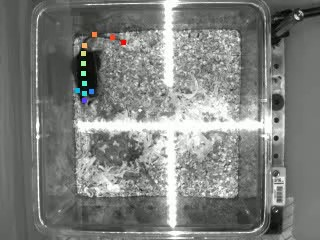
\includegraphics[width=\textwidth, angle=-90]{figures/deeplabcut-top-example-4128-2020-12-02-1-00-37.jpg}
    \caption{}
    \label{fig:deeplabcut-top-example}
  \end{subfigure}
  \begin{subfigure}{0.45\textwidth}
    \centering
    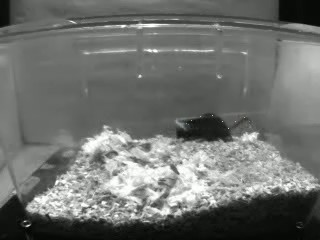
\includegraphics[width=\textwidth]{figures/deeplabcut-lateral-example-4128-2020-12-02-1-00-37.jpg}
    \caption{}
    \label{fig:deeplabcut-lateral-example}
  \end{subfigure}
  \begin{subfigure}{0.45\textwidth}
    \centering
    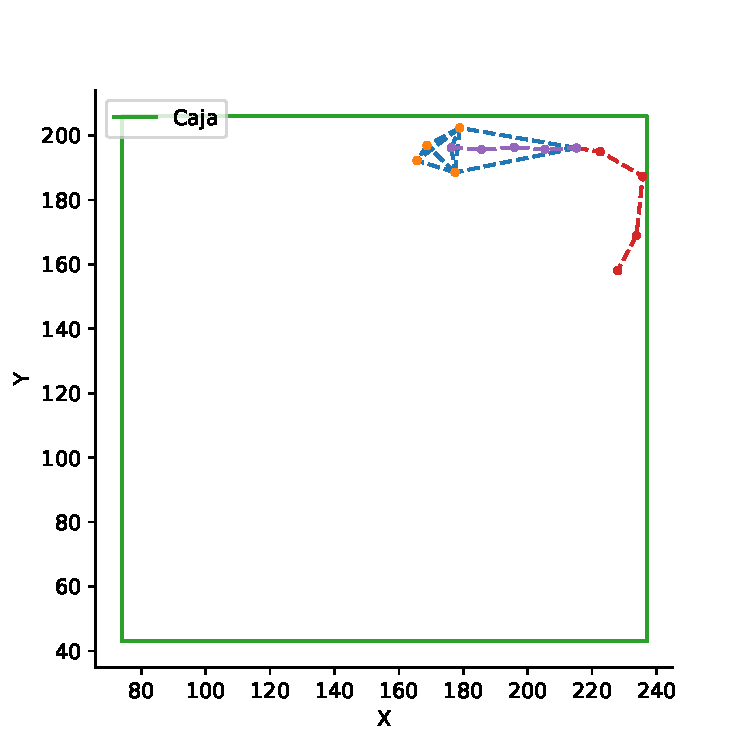
\includegraphics[width=\textwidth]{figures/triangulation-top-4128-2020-12-02.pdf}
    \caption{}
  \end{subfigure}
  \begin{subfigure}{0.45\textwidth}
    \centering
    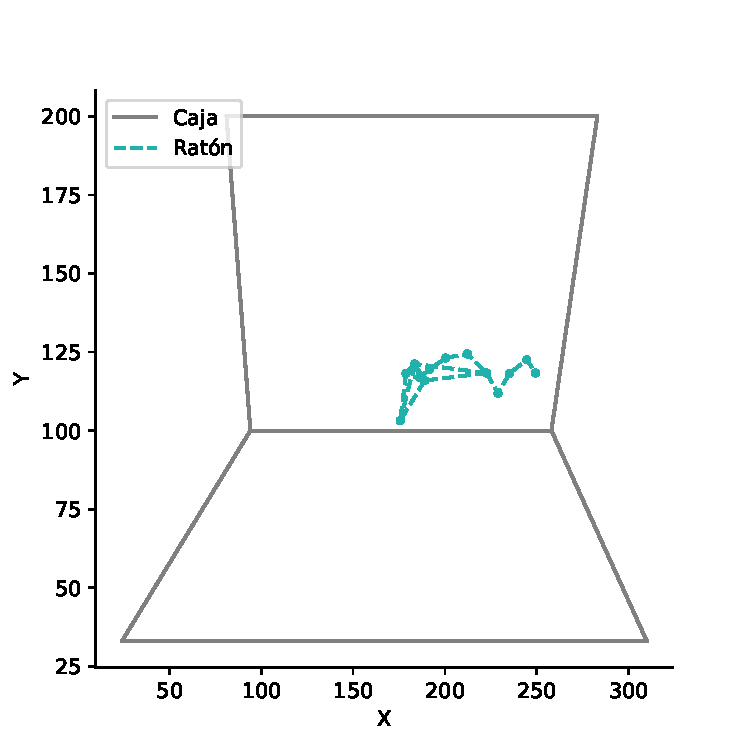
\includegraphics[width=\textwidth]{figures/triangulation-lateral-4128-2020-12-02.pdf}
    \caption{}
  \end{subfigure}
  \caption[Salida de DeepLabCut.]
  {Salida de DeepLabCut del animal 4128 el 02-12-2020, 1:00:37. \ref{fig:deeplabcut-top-example} Video de la vista cenital de la caja. Los puntos sobre el animal son los dibujados por DeepCutLab para rastrear las partes del animal. \ref{fig:deeplabcut-lateral-example} Video de la vista lateral de la caja.}
  \label{fig:deeplabcut-outputexamples}
\end{figure}

% Dataframe example
\begin{table}[]
  \centering
  \begin{tabular}{|c|c|c|c|c|c|c|}
  \hline
    & Nosex & Nosey & Noselikelihood & Headx & Heady & ... \\
  \hline
  0 & 136.165344 & 177.722496 & 0.000084 & 129.790253 & 174.772552 & ... \\
  1 & 162.032005 & 201.444756 & 0.942181 & 168.152061 & 202.420639 & ... \\
  2 & 156.297043 & 200.326378 & 0.000073 & 162.436028 & 203.156837 & ... \\
  3 & 155.370415 & 199.043297 & 0.000277 & 159.507599 & 200.199928 & ... \\
  4 & 149.272644 & 197.677170 & 0.000045 & 155.493912 & 198.814835 & ... \\
  ... & ... & ... & ... & ... & ... & ... \\
  \hline
  \end{tabular}
  \caption[Datos de DeepLabCut]{Extracto del \texttt{DataFrame} de \texttt{pandas} de los datos sin procesar de DeepLabCut. Para cada punto rasteado, y para cada fotograma del video, se computa la predicción de la coordenada $x$ y de la coordenada $y$ y se da la verosimilitud de dicha predicción.}
  \label{tab:df-example}
\end{table}


\subsection{Filtrado e interpolación}

% Raw trayectory
\begin{figure}[H]
  \centering
  \begin{subfigure}{0.45\textwidth}
    \centering
    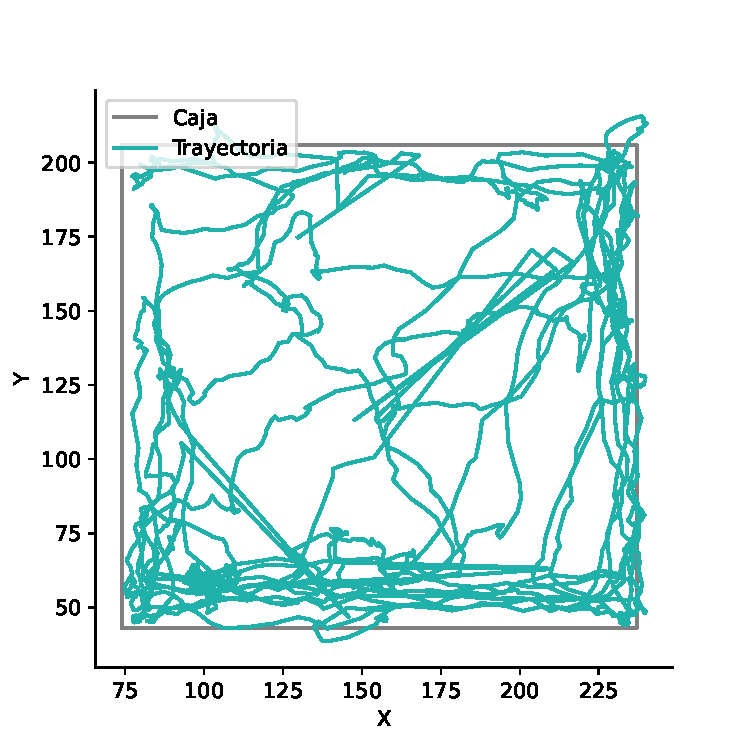
\includegraphics[width=\textwidth]{figures/raw-trayectory-top-4128-2020-12-02.pdf}
    \caption{}
  \end{subfigure}
  \begin{subfigure}{0.45\textwidth}
    \centering
    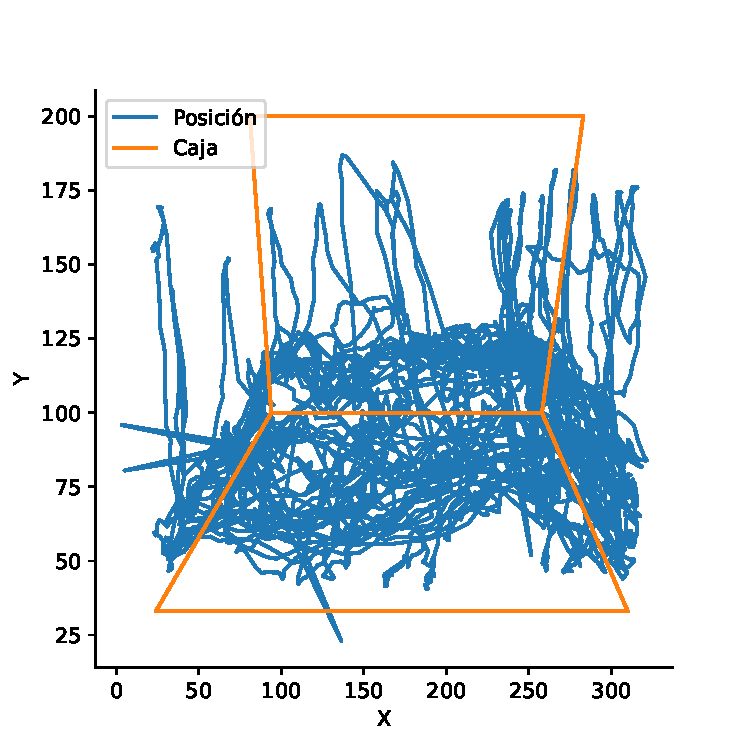
\includegraphics[width=\textwidth]{figures/raw-trayectory-lateral-4128-2020-12-02.pdf}
    \caption{}
    \label{fig:raw-top}
  \end{subfigure}
  \begin{subfigure}{0.45\textwidth}
    \centering
    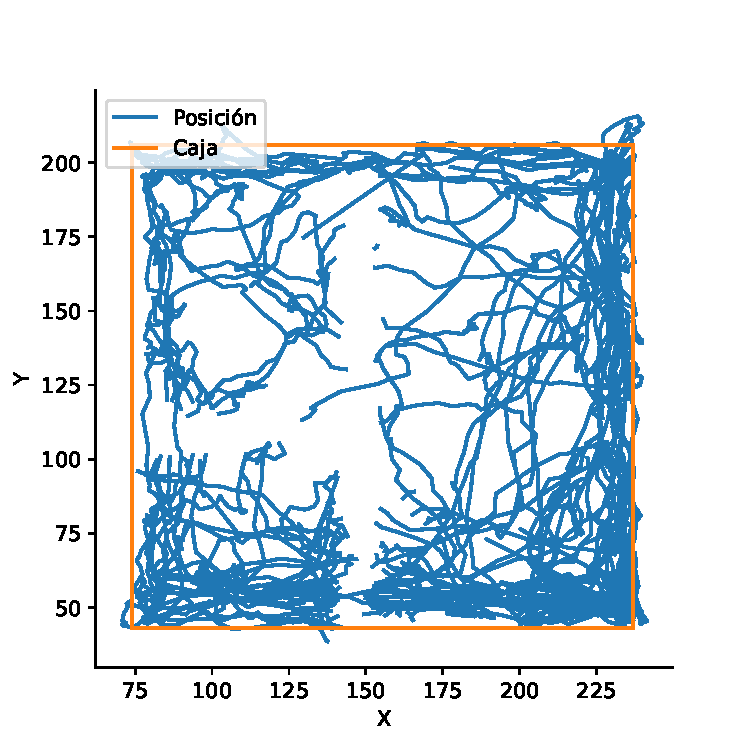
\includegraphics[width=\textwidth]{figures/filtered-trayectory-top-4128-2020-12-02.pdf}
    \caption{}
  \end{subfigure}
  \begin{subfigure}{0.45\textwidth}
    \centering
    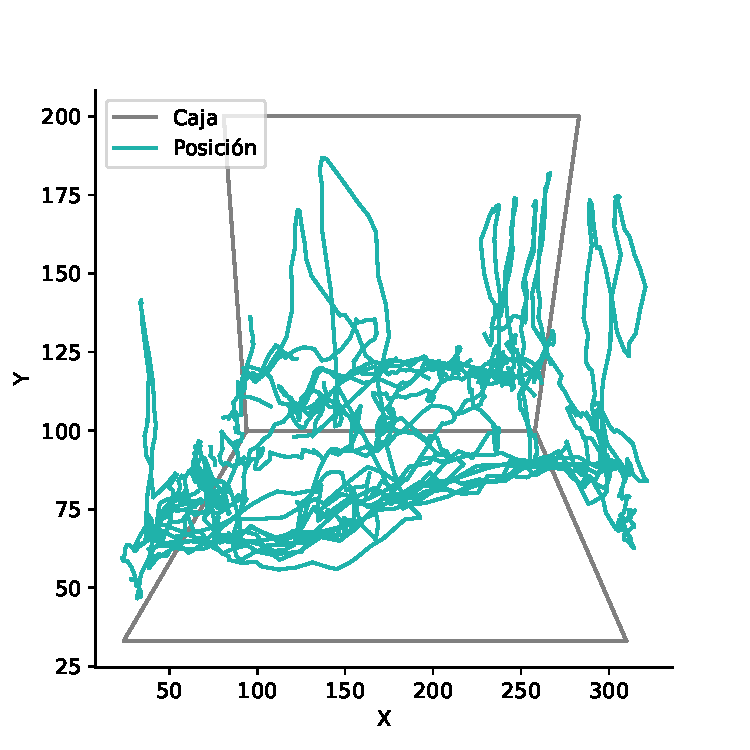
\includegraphics[width=\textwidth]{figures/filtered-trayectory-lateral-4128-2020-12-02.pdf}
    \caption{}
  \end{subfigure}
  \begin{subfigure}{0.45\textwidth}
    \centering
    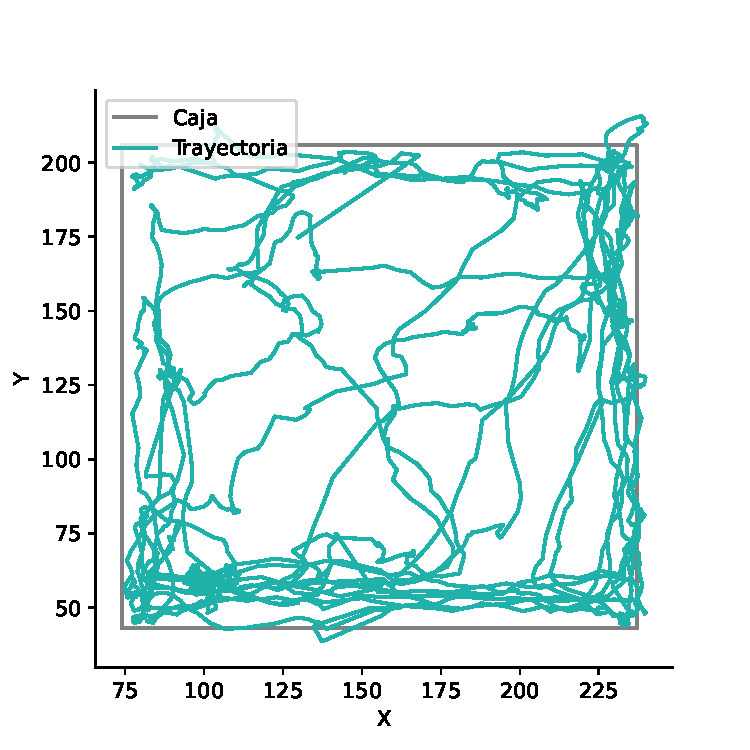
\includegraphics[width=\textwidth]{figures/interpolated-trayectory-top-4128-2020-12-02.pdf}
    \caption{}
  \end{subfigure}
  \begin{subfigure}{0.45\textwidth}
    \centering
    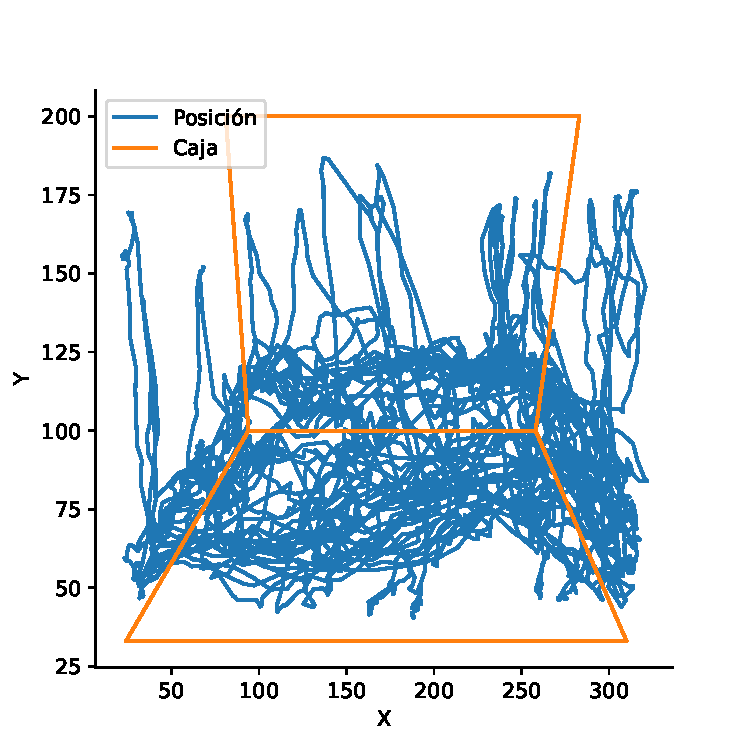
\includegraphics[width=\textwidth]{figures/interpolated-trayectory-lateral-4128-2020-12-02.pdf}
    \caption{}
  \end{subfigure}
  \caption[Trayectorias durante el preprocesado]{Vistas cenital y lateral de trayectorias de un punto de la cabeza del animal. Datos correspondientes a los dos primeros minutos de la sesión del 2020-12-02 del animal 4128. \ref{fig:raw-top}: Vista cenital de los datos antes del preprocesado. En gris se ha dibujado las dimensiones de la caja y en color la trayectoria del punto \texttt{Head}.}
  \label{fig:raw-trayectories}
\end{figure}


\subsection{Computo de variables a analizar}

\newpage
\section{Procesado de datos}

\subsection{Matriz de similitud}

\subsection{Agrupamiento por afinidad}

\subsection{Reducción de dimensionalidad para visualización}

\subsection{Entrenamiento de una red neuronal}
